\documentclass[border=10pt]{standalone}
\usepackage{pgfplots}
\pgfplotsset{compat=1.18}
\begin{document}
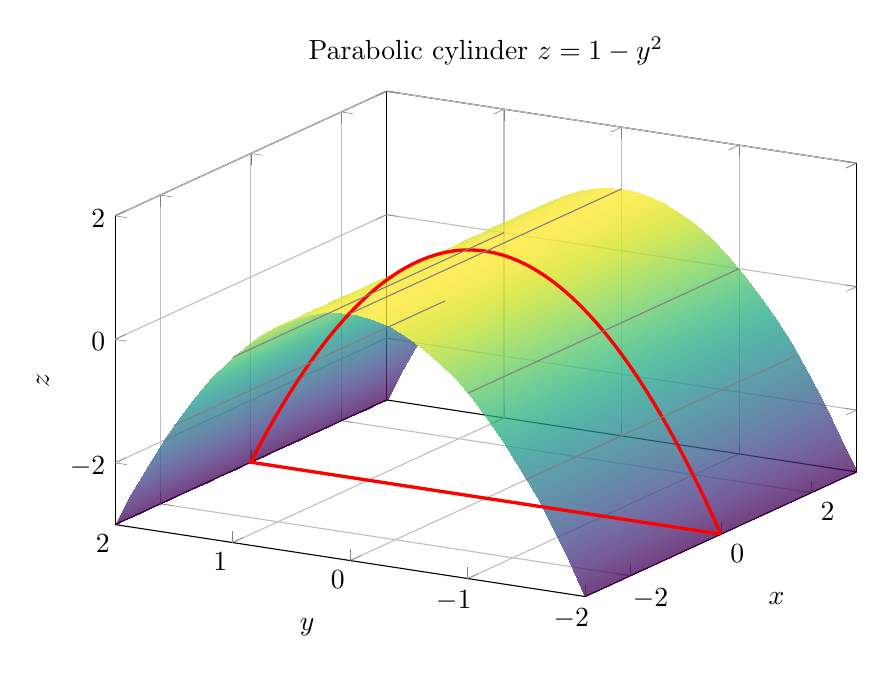
\begin{tikzpicture}
\begin{axis}[
    width=11cm, height=8cm,
    view={-60}{25},
    xlabel={$x$}, ylabel={$y$}, zlabel={$z$},
    title={Parabolic cylinder $z=1-y^2$},
    grid=major,
    zmin=-3, zmax=2,
    xmin=-3, xmax=3,
    ymin=-2, ymax=2,
]
\addplot3[
    surf,
    shader=interp,
    colormap/viridis,
    opacity=0.75,
    domain=-3:3,
    y domain=-2:2,
    samples=30,
    samples y=30
] {1-y^2};
\addplot3[
    red, very thick,
    domain=-2:2,
    samples=80
] (0,x,{1-x^2});
\addplot3[gray, no marks] coordinates {(-3,-1.5,-1.25) (3,-1.5,-1.25)};
\addplot3[gray, no marks] coordinates {(-3,-1,0) (3,-1,0)};
\addplot3[gray, no marks] coordinates {(-3,0,1) (3,0,1)};
\addplot3[gray, no marks] coordinates {(-3,1,0) (3,1,0)};
\addplot3[gray, no marks] coordinates {(-3,1.5,-1.25) (3,1.5,-1.25)};
\end{axis}
\end{tikzpicture}
\end{document}